The generated mesh may still need additional cleanup and detail. The topology is dependend on the used meshing algorithm, naturally. The laser scanner beam cannot sample reflective or transparent structures. It can only provide a great reference for manual tracing.

\section{Modeling the current Pellerhaus facade}

The lower part of the Pellerhaus facade is very similar, almost identical, to the historic one. Thus modeling the modern facade based on LiDAR, photogrammetry and photographic reference appeared to make sense.

\subsection{Using the PC2B converter software}

Firstly, the LiDAR data was preprocesed in PC2B. We created five scans on location, so all scans have been preprocessed and imported into Blender.\parencite{dp_lidar}.

\subsection{Using UAV references with photogrammetry}

Unmanned Aerial Vehicles (UAV's or simply drones) are getting affordable, even very good quality models. In our research we use the DJI Phantom 2 with a GoPro Hero 4 Black mounted on a 3-axis DJI Zenmuse H3-3D Gimbal to create photographic aerial references of the Pellerhaus Nürnberg.

Flying a drone inside the city center of Nuremberg is not as easy, as it might be assumed at first. Before even being able to take off with a UAV, German law requires a general permission for just entering the air space. In addition every UAV pilot needs an UAV insurance.

Regarding the usage of drones in the city center, there are more restrictions. The city center of Nuremberg is covered by the controlled air space. Flying in that air space is not permitted until the starting permission from the bavarian aviation authority and UAV insurance are upgraded to commercial ones. Furthermore pilots need a clearance from the Air traffic control (ATC). Additionally the starting and landing procedure requires to cordon off pedestrians and a special license from the traffic authority. Lastly, the owner of the property needs to be asked for permission to allow the starting and landing of the aircraft.

Luckily there are some laws that permit video shoots and taking photos. For example the Freedom of panorama (§ 59, German Urheberrechtsgesetz) allows taking photos from pavements and roads permanently located in a public place. This right to freely take and share photographs of buildings and works of public art may be abolished on July 9th, 2015 by the European Parliament (see \parencite{freedomOfPanoramaUnderAttack}). We expect immense implications on historic documentation of buildings if this happens.

In total we made three flights on location. It was planned to use the second flight for single photos shot in an interval of 1 second whereas the other two flights are videos in 4K. Unfortunately, it turned out that the third flight wasn't recorded at all and the second flight was captured as a video file. Luckily we noticed the third video missing while still on location, having a bit of battery life left and about one hour left to use the air space, so we made at least two impressive aerial shots before ending the mission.

With having video files instead of still images, those needed to be exported as stil frames to be able to be processed by software. We tried both the free "Visual SfM" and commercial "Agisoft Photoscan Pro" software solutions to generate additional colored meshes of the Pellerhaus. The total processing time of about 20 hours for Visual SfM and 40 hours for Photoscan to get a 3D point cloud from the images. Comparing the results we noticed that Visual SfM generated a bend facade while Photoscan Pro kept it very straight. Although not recommended in (), we used a GoPro camera with a short focal length and thus a strong lens distortion for 3d reconstruction. We can confirm, that the use of this camera is not a good choice, since the radial distortion can produce errors in the feature matching phase of photogrammetry. Still the output should be a good reference for the rough shape of the reconstructed object. If available, LiDAR data should be used for accurate building reconstruction.

\section{Modeling the historic Pellerhaus facade}

Based on the modern facade it was possible to get a good feel for the size of the Pellerhaus in the renaissance. Still the main parts above the ground floor of the facade differ dramatically from the modern one. They can only be extracted from photographs.

\subsection{Using historic images as guide}

It is a huge luck that the Pellerhaus history has been documented by an enormous amount of pictures. A big load of about 190 pictures has been provided for free through the Altstadtfreunde Nürnberg e.V. association, not including about 100 additional pictures depicting the space in front of the building.


\begin{figure}[h]
	\centering
	
\includegraphics[scale=0.4]{graph_a.png}
	\caption{A description}
	\label{fig:something}
\end{figure}

Those pictures can be traced in Blender.

\subsection{Using historic stereoscopic images with photogrammetry}

Although the historic pictures have already been a blessing, there are two images aquired by stereophotography. Trying to feed the left and right image into photogrammetry software, respectively, gives a nice 3d representation of the historic facade already. Of course, little details are still missing.


%\parencite{einstein}
%\parencite[see][p10]{latexcompanion}
%\parencite[compare][]{knuthwebsite}
%\parencite[e.g.][page300]{einstein}
%\parencite{einstein}
%\parencite{einstein}
%\parencite{einstein}




\section{The finished models}



\begin{figure}[h]
	\centering
	\begin{subfigure}[b]{0.45\textwidth}
		\centering
		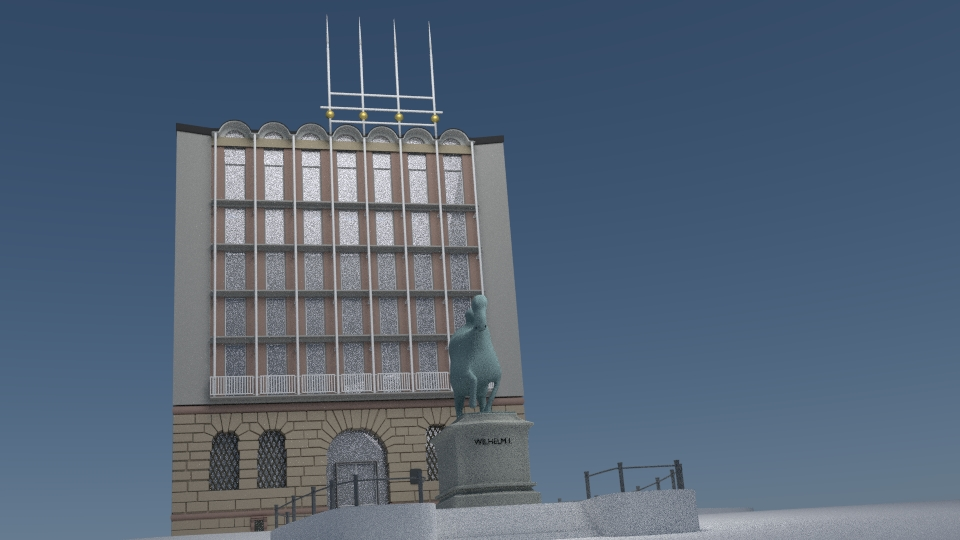
\includegraphics[width=\textwidth]{Pellerhaus_3d_a.jpg}
		\caption{Modern Pellerhaus}
		\label{fig:pellerhaus_3d_modern}
	\end{subfigure}
	\hfill
	\begin{subfigure}[b]{0.45\textwidth}
		\centering
		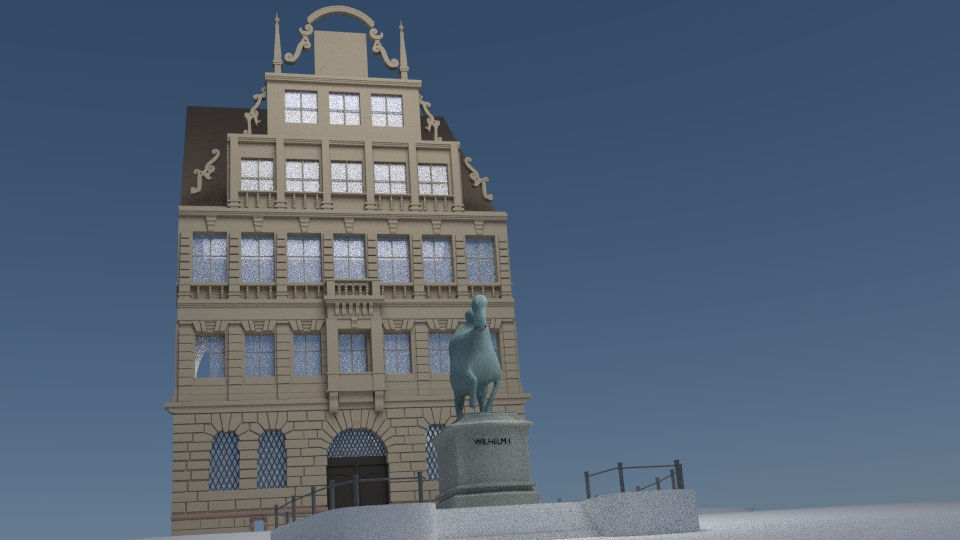
\includegraphics[width=\textwidth]{Pellerhaus_3d_b.jpg}
		\caption{Historic Pellerhaus}
		\label{fig:pellerhaus_3d_historic}
	\end{subfigure}
	\caption{The Pellerhaus modeled manually}
	\label{fig:pellerhaus_3d_models}
\end{figure}







\begin{figure}[h]
	\centering
	\begin{subfigure}[b]{0.45\textwidth}
		\centering
		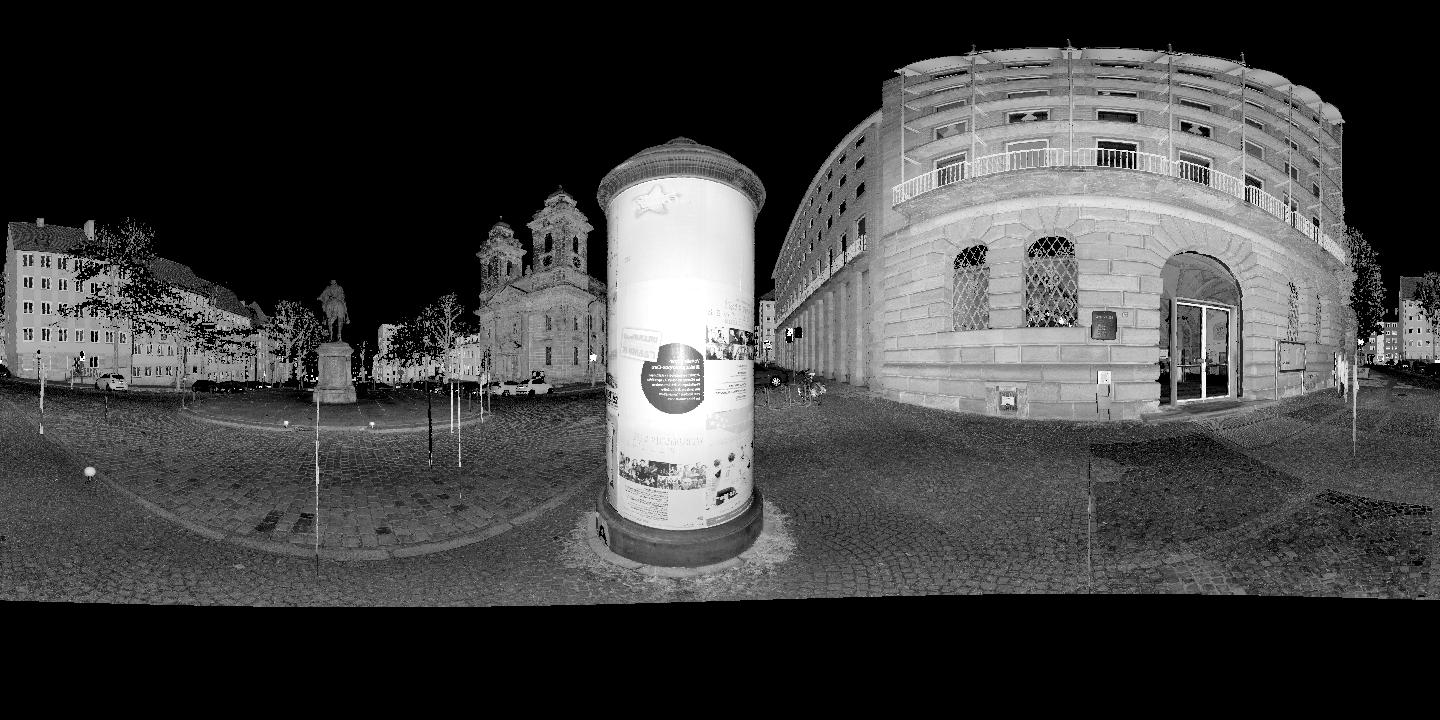
\includegraphics[width=\textwidth]{PC2B_colormap_grey.jpg}
		\caption{Colormap}
		\label{fig:PC2B_colormap_grey}
	\end{subfigure}
	\hfill
	\begin{subfigure}[b]{0.45\textwidth}
		\centering
		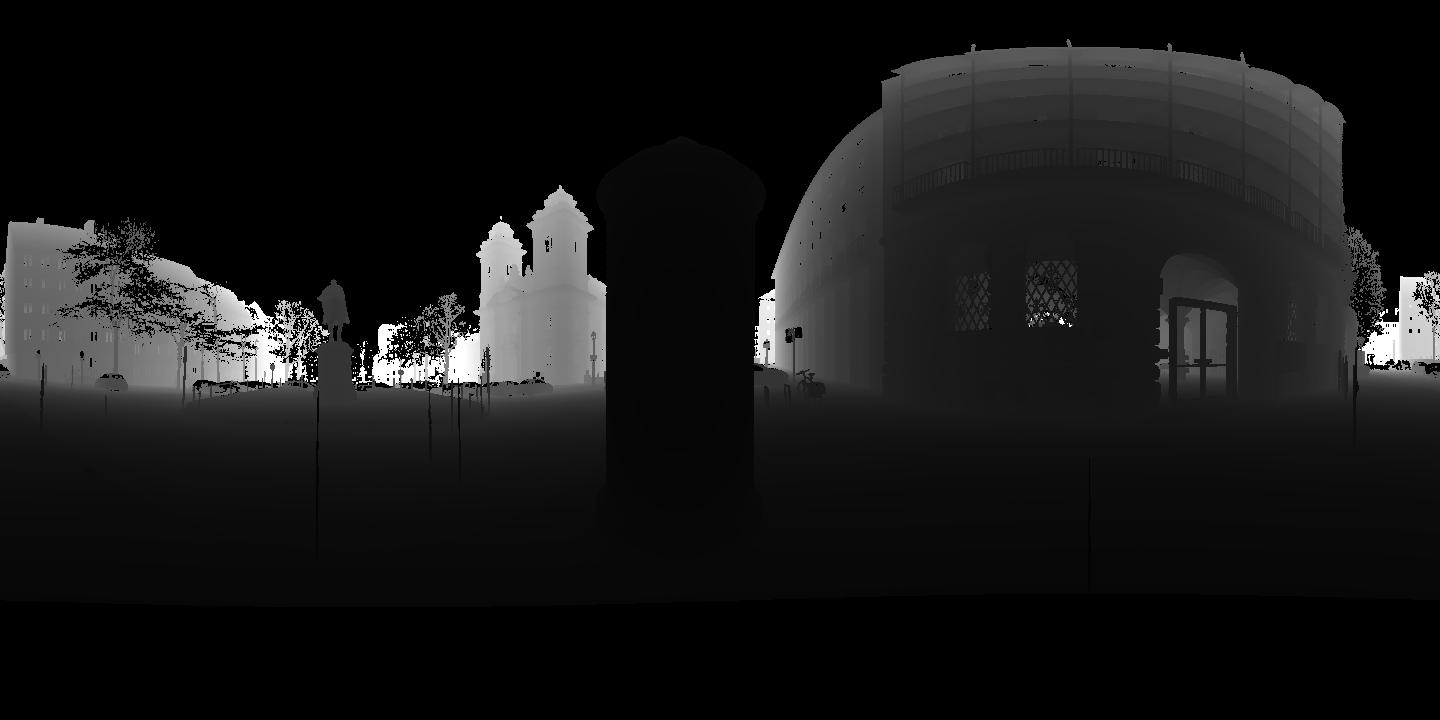
\includegraphics[width=\textwidth]{PC2B_depthmap.jpg}
		\caption{Depthmap}
		\label{fig:PC2B_depthmap}
	\end{subfigure}
	\caption{The Pellerhaus modeled manually}
	\label{fig:pellerhaus_3d_models}
\end{figure}





The modeling process is finished with the creation of the destructed Pellerhaus, which basically only consists of the base floor.[compare][]{webLaTeX-Tutorial}.

\section{Animating between the states}

Since the created models are very similar in size, it is possible to animate a simple fade between them.
A more interesting solution is a fracturing simulation, though.

\section{Lighting and Rendering}

The models need to be evenly lit.

\section{Stereoscopic Rendering as anaglyph 3d}

For a better presentation, the scene can also be visualized in stereoscopic 3d. Through the newly implemented stereo feature in Blender this is now a hassle-free process.